%%%%%%%%%%%%%%%%%%%%%%%%%%%%%%%%%%%%%%%%%%%%%%%%%%%%%%%%%%%%%%%%%%%%%%%%%%%%%%
%
% Chapter: Hadoop MapReduce and Hive Solution
%
%%%%%%%%%%%%%%%%%%%%%%%%%%%%%%%%%%%%%%%%%%%%%%%%%%%%%%%%%%%%%%%%%%%%%%%%%%%%%%
\chapter{Design and Implementation} \label{ch:solution}
The developmental process for the design and implementation of our solutions to the payment history analysis case study is split into two distinct phases: \textit{test data generation} and \textit{solution implementation}. First, we generate our test data using Hadoop MapReduce, which is requisite to benchmarking each solution we implement. Second, we implement the RDBMS solution as a control in MySQL, followed by two DDMS solutions: Hadoop MapReduce and Hive.

\section{Test Data Generation Phase}
Before we can evaluate the scalability of each implementation, we need to generate large data sets based on the sample data provided by CompanyX. For each solution, the performance depends highly on the complexity of the relationships between customer, account, and transaction data. Therefore, it is crucial to maintain the probability distribution relationships of the sample data so we may achieve accurate and comparable benchmark results. For this, we introduce a package of test data generation utilities.

First, the \texttt{HistogramGen} MapReduce program identifies the probability distribution relationships for a subject sample data set. Second, the \texttt{HistogramGen} output is supplied as input to the \texttt{AccountGen} utility, which generates the test data sets.

\subsection{HistogramGen: Statistical Analysis of Sample Data}
The \texttt{HistogramGen} utility determines the probability distribution of the sample data set and generates a histogram report. Since performance depends on relationship complexity between account and customer data, we evaluate averages based on the number of:
\begin{enumerate}
 \item accounts per customer,
 \item customers per SSN,
 \item charge, adjustment, and payment transactions per account, and
 \item charge, adjustment, and payment transactions per strategy history.
\end{enumerate}

Figure~\ref{fig:histogen} provides an overview the \texttt{HistogramGen} program flow described below.

\begin{figure}[hc]
% \begin{figure}[hct!]
 \centering
 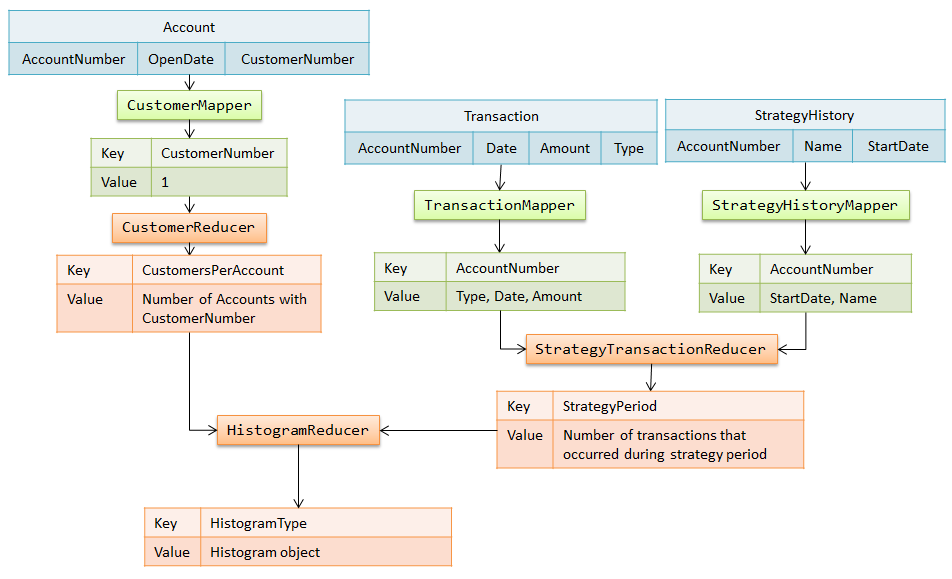
\includegraphics[scale=0.60]{../images/HistogramGen.png}
 % StageOne.png: 931x454 pixel, 96dpi, 24.64x12.01 cm, bb=0 0 698 341
  \caption{\texttt{HistogramGen} program flow diagram}
  \label{fig:histogen}
\end{figure}

The number of accounts per customer is determined by counting the number of \texttt{Account} entries with the same \texttt{CustomerNumber} attribute. This sum is found with the simple map and reduce methods shown below. The \texttt{CustomerMapper} takes each \texttt{Account} entry as input and maps the \texttt{CustomerNumber} for the account to a value of $1$. 
%   public static class CustomerMapper extends MapReduceBase 
%     implements Mapper<Object, Text, Text, IntWritable> 
%     {
%       public static final int COL_ACCOUNT_NUM = 0;
%       public static final int COL_OPEN_DATE = 1;
%       public static final int COL_CUSTOMER_NUM = 2;
%       public static final IntWritable ONE = new IntWritable(1);
% 
%       public void map(Object offset, Text input, 
%         OutputCollector<Text, IntWritable> output,
%         Reporter reporter) throws IOException 
%       {
%         String[] parts = (input.toString()).split(",");
%         String customerNumber = parts[COL_CUSTOMER_NUM].trim();
%         output.collect(new Text(customerNumber), ONE);
%       }
%   } 
{
\singlespace
\small
\begin{verbatim}
public void map(Object offset, Text input, 
     OutputCollector<Text, IntWritable> output, Reporter reporter) 
     throws IOException 
{
    String[] parts = (input.toString()).split(",");
    String customerNumber = parts[COL_CUSTOMER_NUM].trim();
    output.collect(new Text(customerNumber), ONE);
}
\end{verbatim}
}
The \texttt{CustomerReducer} receives the mapped output for each \texttt{CustomerNumber} key from the \texttt{CustomerMapper} and sums the value of each to get the total number of accounts for the \texttt{CustomerNumber} key. The resulting output is the total number of accounts for the customer mapped to the histogram type. 
%   public static class CustomerReducer extends MapReduceBase implements    
%     Reducer<Text, IntWritable, IntWritable, IntWritable> 
%   {
%     public static final IntWritable histogramType 
%             = new IntWritable(HistogramType.CUSTOMERS_PER_ACCOUNT.ordinal());
% 
%     public void reduce(Text customerNumber, Iterator<IntWritable> values,
%       OutputCollector<IntWritable, IntWritable> output,
%       Reporter reporter) throws IOException 
%     {
%       int count = 0;
%       while (values.hasNext())
%       {
%         count += values.next().get();
%       }
%       /* output the type of histogram and the count */
%       output.collect(histogramType, new IntWritable(count));
%     }
%   }
{
\singlespace
\small
\begin{verbatim}
public void reduce(Text customerNumber, Iterator<IntWritable> values,
      OutputCollector<IntWritable, IntWritable> output,
      Reporter reporter) throws IOException 
{
    int count = 0;
    while (values.hasNext())
    {
        count += values.next().get();
    }
    /* output the type of histogram and the count */
    output.collect(histogramType, new IntWritable(count));
}
\end{verbatim}
}

Furthermore, since performance depends on relationship complexity between the transaction data, the number of queries also depends on the strategy history and type of transaction for each strategy. Therefore, we evaluate the number of good standing and bad debt charges, adjustments, and payments per account. For each account, the number of transactions per strategy history are determined by counting the number of {\tt Transaction} entries with the same {\tt AccountNumber} attribute and the number of {\tt Transactions} that occur during each {\tt StrategyHistory} period. These sums are found with the simple map and reduce methods shown below. 

The {\tt TransactionMapper} maps the {\tt Transaction} to the owning {\tt AccountNumber}.
%  public static class TransactionMapper extends MapReduceBase implements 
%     Mapper<Object, Text, Text, ObjectWritable> 
%   {
%     public static final int COL_ACCOUNT_ID = 0;
%     public static final int COL_DATE = 1;
%     public static final int COL_AMOUNT = 2;
%     public static final int COL_TYPE = 3;
% 
%     public void map(Object offset, Text input,
%         OutputCollector<Text, ObjectWritable> output, Reporter reporter)
%         throws IOException 
%     {
%       String[] parts = input.toString().split(",");
%       String account = parts[COL_ACCOUNT_ID].trim();
%       String date = parts[COL_DATE].trim();
%       String amount = parts[COL_AMOUNT].trim();
%       String type = parts[COL_TYPE].trim();
% 
%       /* Output transactions by accountNumber */
%       Transaction transaction = new Transaction(date, type, amount);
%       output.collect(new Text(account), new ObjectWritable(transaction));
%     }
%   }
{
\singlespace
\small
\begin{verbatim}
public void map(Object offset, Text input, 
     OutputCollector<Text, ObjectWritable> output, Reporter reporter) 
     throws IOException 
{
    String[] parts = input.toString().split(",");
    String account = parts[COL_ACCOUNT_ID].trim();
    String date = parts[COL_DATE].trim();
    String amount = parts[COL_AMOUNT].trim();
    String type = parts[COL_TYPE].trim();

    /* Output transactions by accountNumber */
    Transaction transaction = new Transaction(date, type, amount);
    output.collect(new Text(account), new ObjectWritable(transaction));
}
\end{verbatim}
}
The {\tt StrategyMapper} maps the {\tt StrategyHistory} to the owning {\tt AccountNumber}.
%   public static class StrategyHistoryMapper extends MapReduceBase implements
%     Mapper<Object, Text, Text, ObjectWritable> 
%   {
%     public static final int COL_ACCOUNT_ID = 0;
%     public static final int COL_NAME = 1;
%     public static final int COL_DATE = 2;
% 
%     public void map(Object offset, Text input,
%       OutputCollector<Text, ObjectWritable> output, Reporter reporter)
%       throws IOException 
%     {
%       String[] parts = (input.toString()).split(",");
%       String account = parts[COL_ACCOUNT_ID].trim();
%       String name = parts[COL_NAME].trim();
%       String startDate = parts[COL_DATE].trim();
% 
%       /* Output strategy history by accountNumber */
%       StrategyHistory strategy = new StrategyHistory(startDate, name);
%       output.collect(new Text(account), new ObjectWritable(strategy));
%     }
%   }
{
\singlespace
\small
\begin{verbatim}
public void map(Object offset, Text input, 
    OutputCollector<Text, ObjectWritable> output, Reporter reporter)
    throws IOException 
{
    String[] parts = (input.toString()).split(",");
    String account = parts[COL_ACCOUNT_ID].trim();
    String name = parts[COL_NAME].trim();
    String startDate = parts[COL_DATE].trim();

    /* Output strategy history by accountNumber */
    StrategyHistory strategy = new StrategyHistory(startDate, name);
    output.collect(new Text(account), new ObjectWritable(strategy));
}
\end{verbatim}
}
The {\tt StrategyTransactionReducer} accepts key/value pairs from the\\ {\tt TransactionMapper} and {\tt StrategyHistoryMapper}, iterates through the list of events for the key account, and sums the values for each account. The output is the number of each transaction type per {\tt AccountNumber}.
{
\singlespace
\small
\begin{verbatim}
public void reduce(Text key, Iterator<ObjectWritable> values,
        OutputCollector<IntWritable, IntWritable> output, Reporter reporter)
        throws IOException 
{
    /* Keep list of payments */
    List<EventWritable> events = new ArrayList<EventWritable>();

    /* Keep track of strategy dates */
    Calendar goodStrategy = new GregorianCalendar();
    Calendar badDebt = new GregorianCalendar();

    while (values.hasNext()) 
    {
        EventWritable next = (EventWritable)        
        values.next().get();
        String type = next.getType().toString();
        events.add(next);
        /* Set good standing dates */
        if (type.equals(StrategyHistory.GOOD_STANDING)) 
        {
          //create event for 30, 60, 90 day after strategy starty date 
        }
        /* Set bad debt dates */
        else if (type.equals(StrategyHistory.BAD_DEBT)) 
        {
          //create event for 30, 60, 90 day after strategy starty date
        }
    }
        
    /* Sort by date and find sums */
    Collections.sort(events);
    for(EventWritable event : events) 
    {
        // count transactions per event strategy
    }

    // output one for each event strategy
    for(int i = 0; i < strategy_counts.length; i++)
    {
        output.collect(new IntWritable(i),newIntWritable(strategy_counts[i]));
    }
 }
\end{verbatim}
}

Finally, the {\tt HistogramReducer} consolidates the resulting output from the \\{\tt CustomerReducer} and {\tt StrategyTransactionReducer} into the final histogram.
{
\singlespace
\small
\begin{verbatim}
public void reduce(IntWritable key, Iterator<IntWritable> values,
        OutputCollector<Text, Histogram> output, Reporter reporter)
        throws IOException 
{
    /* What type of histogram is this? */
    HistogramType type = HistogramType.getType(key.get());

    /* add all the values to a temp list */
    ArrayList<Integer> temp = new ArrayList<Integer>();	
    while (values.hasNext()) 
    {
        temp.add(values.next().get());
    }

    /* sort list and create a new Histogram from data */
    Collections.sort(temp);
    Histogram histogram = new Histogram(type, temp.toArray(new Integer[0]));
    output.collect(new Text(type.toString()), histogram);
}
\end{verbatim}
}

\subsection{AccountGen: Test Data Generation}
The {\tt AccountGen} program uses the {\tt HistogramGen} probability distribution results to generate the test data sets with the {\tt Customer}, {\tt Account}, {\tt Transaction}, and {\tt StrategyHistory} entries. 

To decrease time requirements for generating large data sets, the work load is distributed among several mappers. For this, we define our own {\tt InputSplit} and {\tt RecordReader} to send an account number range to each mapper. Then for each account, the mapper uses the histogram statistics to determine:
\begin{enumerate}
 \item which {\tt CustomerNumber} to assign, and
 \item how many of each transaction type to generate (with the account number as the primary key).
\end{enumerate}

The {\tt MultipleOutputFormat} provided in the MapReduce API is used to output each entry (customer, account, transaction, strategy history) to a separate, comma-separated file. The attributes remain the same as the original entries. 

\section{MySQL Solution}
Since CompanyX already has a RDBMS implementation of the payment history analysis case study in place, we were able to leverage the existing SQL script used to pull expected results for the desired output file from tables in our MySQL solution. We developed the MySQL solution in the following steps:
\begin{enumerate}
 \item Define schema for payment history analysis database.
 \item Implement MySQL script to load account, customer, transaction and strategy history data into database tables.
 \item Update existing SQL script to execute in MySQL.
\end{enumerate}
We were able to derive the table definitions, data types, and constraints for the database schema from the provided background data and SQL query (see Appendix~\ref{app:mysql} for complete schema). Since we will be generating new data sets for each benchmark execution, we need to be able to dynamically load data into the MySQL database. Thus, we implemented a script to generate the MySQL load script based on a given input directory. The final load script is a series of statements of the following form-- \texttt{'load data local infile <filename>  into table <table name>'}. Finally, upon executing the SQL script in MySQL, we quickly realized that the existing SQL script used to pull expected results was not fully compatible with MySQL. So, the final step was to transform the incompatible queries to the MySQL standard and ensure that the result table matched the expected output table.

\section{Hadoop MapReduce Solution}
The MapReduce solution requires three map and reduce phases that are detailed in the following sections. 

\subsection{Stage 1: Customer Join Account}
The first stage combines the Customer and Account tables on the CustomerNumber using a \texttt{CustomerMapper}, \texttt{AccountMapper} and \texttt{CustomerJoinAccountReducer} (see Figure~\ref{fig:stage1}). 

\begin{figure}[hct]
% \begin{figure}[hct!]
 \centering
 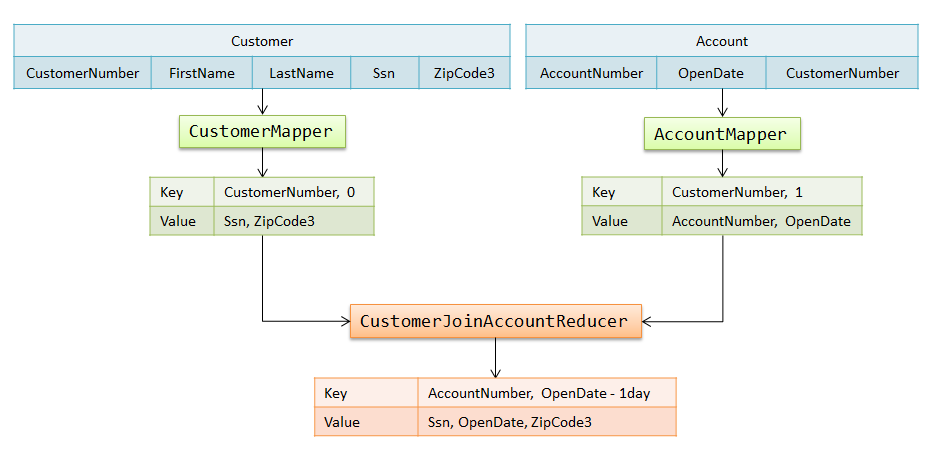
\includegraphics[scale=0.60,bb=0 0 698 341]{../images/StageOne.png}
 % StageOne.png: 931x454 pixel, 96dpi, 24.64x12.01 cm, bb=0 0 698 341
  \caption{Stage 1: Customer join Account program flow diagram}
  \label{fig:stage1}
\end{figure}

% \begin{description}
% \item[\textbf{Customer Mapper}]%\hspace*{\fill} \\
\subsubsection{Customer Mapper}
  \begin{itemize}
  \item The input is the \texttt{Customer} data (formatted as a .csv file). 
  \item The output key is \texttt{CustomerNumber} and the sort order for the key is \texttt{0}.
  \item The output value is \texttt{Ssn} and \texttt{ZipCode3} of the customer.
  \end{itemize}
{
\singlespace
\small
\begin{verbatim}
public void map(Object offset, Text input, 
    OutputCollector<TextPair, Text> output, Reporter reporter) 
    throws IOException {
    
    String[] parts = (input.toString()).split(",");

    String customerNumber = parts[COL_CUSTOMER_NUM].trim();
    String ssn = parts[COL_SSN].trim();
    String zipCode3 = parts[COL_ZIP_CODE_3].trim();

    key.set(new Text(customerNumber), ZERO);
    value = new Text(ssn + "," + zipCode3);

    output.collect(key, value);
}
\end{verbatim}
}
% \item[\textbf{Account Mapper}]\hspace*{\fill} \\
\subsubsection{Account Mapper}
  \begin{itemize}
  \item The input is the \texttt{Account} data (formatted as a .csv file).
  \item The output key is \texttt{CustomerNumber} and the sort order for the key is \texttt{1}.
  \item The output value is \texttt{AccountNumber} and \texttt{OpenDate} of the account.
  \end{itemize}
{
\singlespace
\small
\begin{verbatim}
public void map(Object offset, Text input,
    OutputCollector<TextPair, Text> output, Reporter reporter) 
    throws IOException {

    String[] parts = (input.toString()).split(",");

    String accountNumber = parts[COL_ACCOUNT_NUM].trim();
    String openDate = parts[COL_OPEN_DATE].trim();
    String customerNumber = parts[COL_CUSTOMER_NUM].trim();

    key.set(customerNumber, "1");
    value = new Text(accountNumber + "," + openDate);
    output.collect(key, value);
}
\end{verbatim}
}
% \item[\textbf{Customer JOIN Account Reducer}]\hspace*{\fill} \\
\subsubsection{Customer Join Account Reducer}
  \begin{itemize}
  \item The input is the sorted output from the Customer and Account mappers. Since the key value of each Customer is unique and the sort order for the
  Customer is 0, the Customer will be the first input value followed by a list of Accounts owned by the Customer. 
  \item The output key is \texttt{AccountNumber} and the sort order for the key is \texttt{OpenDate}.
  \item The output value is
    \begin{itemize}
	 \item \texttt{Ssn},
	 \item \texttt{OpenDate}, and
	 \item \texttt{ZipCode3}.
    \end{itemize}
  \end{itemize}
% \end{description}

\subsection{Stage 2: Strategy History Join Transaction}
The second stage combines the Account and Customer data from stage 1 and the Strategy History and Transaction tables on the AccountNumber. This process requires the output from stage one and a \texttt{StrategyHistoryMapper}, \texttt{TransactionMapper} and\\ \texttt{CustomerJoinAccountReducer} (see Figure~\ref{fig:stage2}). 

\begin{figure}[htc!]
 \centering
 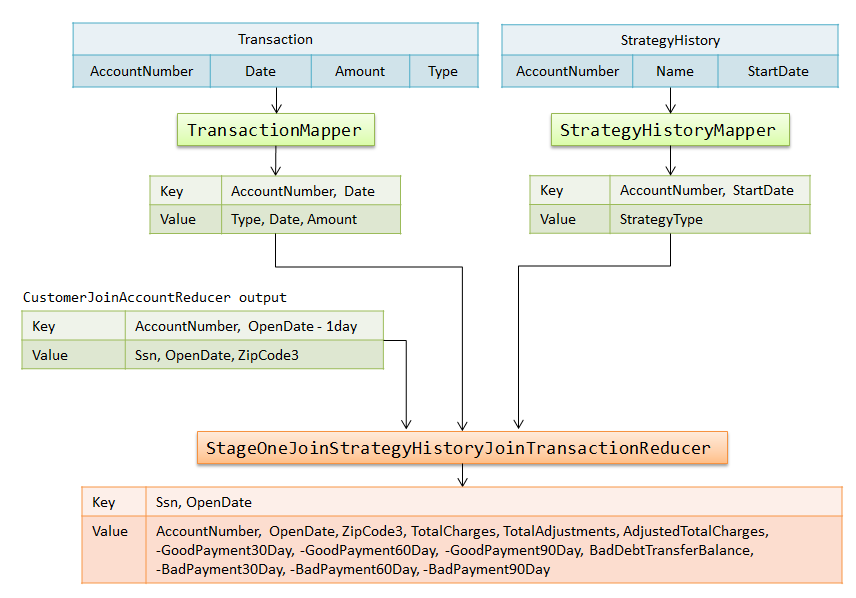
\includegraphics[scale=0.60,bb=0 0 698 341]{../images/StageTwo.png}
 % StageOne.png: 931x454 pixel, 96dpi, 24.64x12.01 cm, bb=0 0 698 341
  \caption{Stage 2: Stragety History join Transaction program flow diagram}
  \label{fig:stage2}
\end{figure}

\subsubsection{Strategy History Mapper}
\begin{itemize}
 \item The input is the \texttt{Strategy History} data (formatted as a .csv
file).
 \item The output key is \texttt{AccountNumber} and the sort order for the key is \texttt{StrategyStartDate}.
 \item The output value is \texttt{StrategyName} of the strategy history. 
\end{itemize}
Note that multiple key/value pairs are output from this mapper. The pair for the strategy start date is output followed by a pair for each of thirty, sixty, and ninety days after the strategy start date.

{
\singlespace
\small
\begin{verbatim}
public void map(Object offset, Text input, 
    OutputCollector<TextDatePair, Text> output, Reporter reporter) 
    throws IOException {

    String[] parts = (input.toString()).split(",");

    String accountNumber = parts[COL_ACCOUNT_NUMBER].trim();
    String name = parts[COL_NAME].trim();
    int type = StrategyType.getByName(name).getNumberOfDays();

    calendar.setTime(DateWritable.df.parse(parts[COL_DATE].trim()));

    key.set(accountNumber, calendar.getTime());
    value.set(Integer.toString(type));
    output.collect(key, value);

    calendar.add(Calendar.DAY_OF_MONTH, 30);
    key.set(accountNumber, calendar.getTime());
    value.set(Integer.toString(type + 1));
    output.collect(key, value);

    calendar.add(Calendar.DAY_OF_MONTH, 30);
    key.set(accountNumber, calendar.getTime());
    value.set(Integer.toString(type + 2));
    output.collect(key, value);

    calendar.add(Calendar.DAY_OF_MONTH, 30);
    key.set(accountNumber, calendar.getTime());
    value.set(Integer.toString(type + 3));
    output.collect(key, value);
}
\end{verbatim}
}

\subsubsection{Transaction Mapper}
\begin{itemize}
 \item The input is the \texttt{Transaction} data (formatted as a .csv file).
 \item The output key is \texttt{AccountNumber} and the sort order for the key is \texttt{TransactionDate}.
 \item The output value is
  \begin{itemize}
    \item \texttt{TransactionType},
    \item \texttt{TransactionDate}, and
    \item \texttt{TransactionAmount} of the transaction.
  \end{itemize}
\end{itemize}.
{
\singlespace
\small
\begin{verbatim}
public void map(Object offset, Text input, 
    OutputCollector<TextDatePair, Text> output, Reporter reporter) 
    throws IOException {

    String[] parts = input.toString().split(",");

    String accountNumber = parts[COL_ACCOUNT_ID].trim();
    String date = parts[COL_DATE].trim();
    String amount = parts[COL_AMOUNT].trim();
    int type = TransactionType.getByName(parts[COL_TYPE].trim()).getOffset();

    key.set(accountNumber, date);
    value.set(type + "," + date + "," + amount);

    output.collect(key, value);
}
\end{verbatim}
}
\subsubsection{Strategy History Join Transaction Reducer}
\begin{itemize}
 \item The input is the sorted output from phase 1 and the Strategy History and
Transaction mappers. Since the output from phase 1 is sorted by the
OpenDate of the Account, it will always be first (because the account must
be opened before any Strategy History or Transactions exist). Also, the key of
each Strategy History is unique and the sort order for both the Strategy History
and Transaction values are by date, so the Transaction values will be separated
into each strategy time period (thirty, sixty, and ninety day) by the Strategy
History values.
 \item The output key is \texttt{Ssn} and the sort order for the key is \texttt{OpenDate}.
 \item The output value is
  \begin{itemize}
  \item \texttt{AccountNumber},
  \item \texttt{OpenDate},
  \item \texttt{ZipCode3},
  \item \texttt{TotalCharges},
  \item \texttt{TotalAdjustments},
  \item \texttt{AdjustedTotalCharges},
  \item \texttt{TotalGoodStandingPayments30Day},
  \item \texttt{TotalGoodStandingPayments60Day},
  \item \texttt{TotalGoodStandingPayments90Day},
  \item  \texttt{BadDebtTransferBalance},
  \item \texttt{TotalBadDebtPayments30Day}, 
  \item \texttt{TotalBadDebtPayments60Day}, and
  \item \texttt{TotalBadDebtPayments90Day}.
  \end{itemize}
\end{itemize}

\subsection{Stage 3: Combine Results}
The final stage uses the output from stage 2 to gather the previous account data for each account (see Figure~\ref{fig:stage3}).

\begin{figure}[htc!]
 \centering
 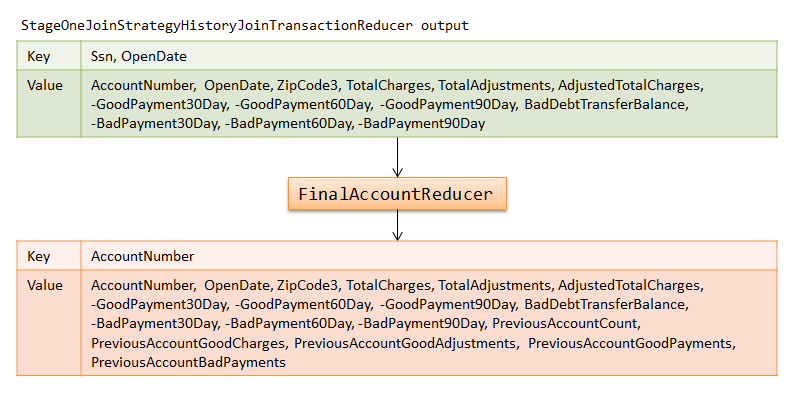
\includegraphics[scale=0.60,bb=0 0 698 341]{../images/StageThree.png}
 % StageOne.png: 931x454 pixel, 96dpi, 24.64x12.01 cm, bb=0 0 698 341
 \caption{Stage 3: Combine results program flow diagram}
 \label{fig:stage3}
\end{figure}

\subsubsection{Identity Mapper}
\begin{itemize}
 \item The input is the sorted output from stage 2. 
 \item The output key is \texttt{AccountNumber}.
 \item The output value is the output value from stage 2 followed by 
   \begin{itemize}
    \item \texttt{PreviousAccountCount},
    \item \texttt{PreviousAccountGoodStandingCharges},
    \item \texttt{PreviousAccountGoodStandingAdjustments},
    \item \texttt{PreviousAccountGoodStandingPayments}, and
    \item \texttt{PreviousAccountBadDebtPayments}.
    \end{itemize}
\end{itemize}

\section{Hive Solution}
Because the HQL syntax is similar to the SQL syntax, we could also leverage CompanyX's existing SQL script for our Hive solution. Similar to the MySQL solution, the steps required for this implementation are:

\begin{enumerate}
 \item Define schema for payment history analysis database.
 \item Implement HQL script to load account, customer, transaction and strategy history data into database tables.
 \item Transform existing SQL script to HQL for Hive execution.
\end{enumerate}

In our case, the major difference between the Hive and MySQL database schema is the additional \texttt{CLUSTERED BY} parameter provided for each table definition. For each table defined in the schema, we cluster by the primary key column into 4 buckets. As in the MySQL solution, we dynamically generate the HQL load script based on a given input directory. The final load script is a series of statements of the following form-- \texttt{'load data inpath <filename> into table <table name>'}. The HQL database schema can be found in Appendix~\ref{app:hive}. 